\section{Results}

Descriptive statistics for hospital processes and patient populations are shown in the supplementary material.

\subsection{Thrombolysis decision model}

The thrombolysis decision model predicted the probability of any patient receiving thrombolysis at any given stroke team.

Using a 80:20 train:test split, the model had an accuracy of 85\%, a balanced accuracy of 82\% (accuracy and balanced accuracy using a 50\% probability cut-off to classify a patient as a binary 'likely to receive thrombolysis' or not), and a receiver operating characteristic area under curve of 0.92.


\subsection{Stroke outcome machine learning model}

Using a 4:1 train:test split, the model had a receiver operating characteristic area under curve of 0.80.

\subsection{Benchmark stroke teams and benchmark decisions}

\textit{Benchmark decisions} are those that would likely be taken by the majority 25 \textit{benchmark} stroke teams most likely to use thrombolysis (if all stroke teams saw the same patients). If all decisions-to-treat were made according to benchmark decisions, average thrombolysis across stroke teams would increase from 36\% to 45\% (in the modelled patient population). Thrombolysis use in the 25 stroke teams least likely to use thrombolysis would increase from 29\% to 46\%.

\subsection{Prototype patients}

\subsubsection{Thrombolysis decisions in prototype patients}

Prototype patients revealed variation in likely decisions between stroke teams (figure \ref{fig:thrombolysis_rates_prototype_patients}). While almost all stroke teams would give thrombolysis to the \textit{ideal} candidate for thrombolysis, the predicted use of thrombolysis varied more as one characteristic was changed from the \textit{ideal} candidate. In particular there was was a very wide range in likelihood of a patient with a mild stroke (NIHSS 3) receiving thrombolysis. Mild stroke (NIHSS 0-4) represents a large proportion of admissions (54\% of all emergency stroke admissions, and 38\% of ischaemic stroke patients arriving by ambulance within 4 hours of known stroke onset). Combinations of \textit{non-ideal} patient characteristics reduced predicted use of thrombolysis further (again with significant variation between stroke teams), especially when the non-ideal characteristic was a mild stroke.

\begin{figure}
    \centering
    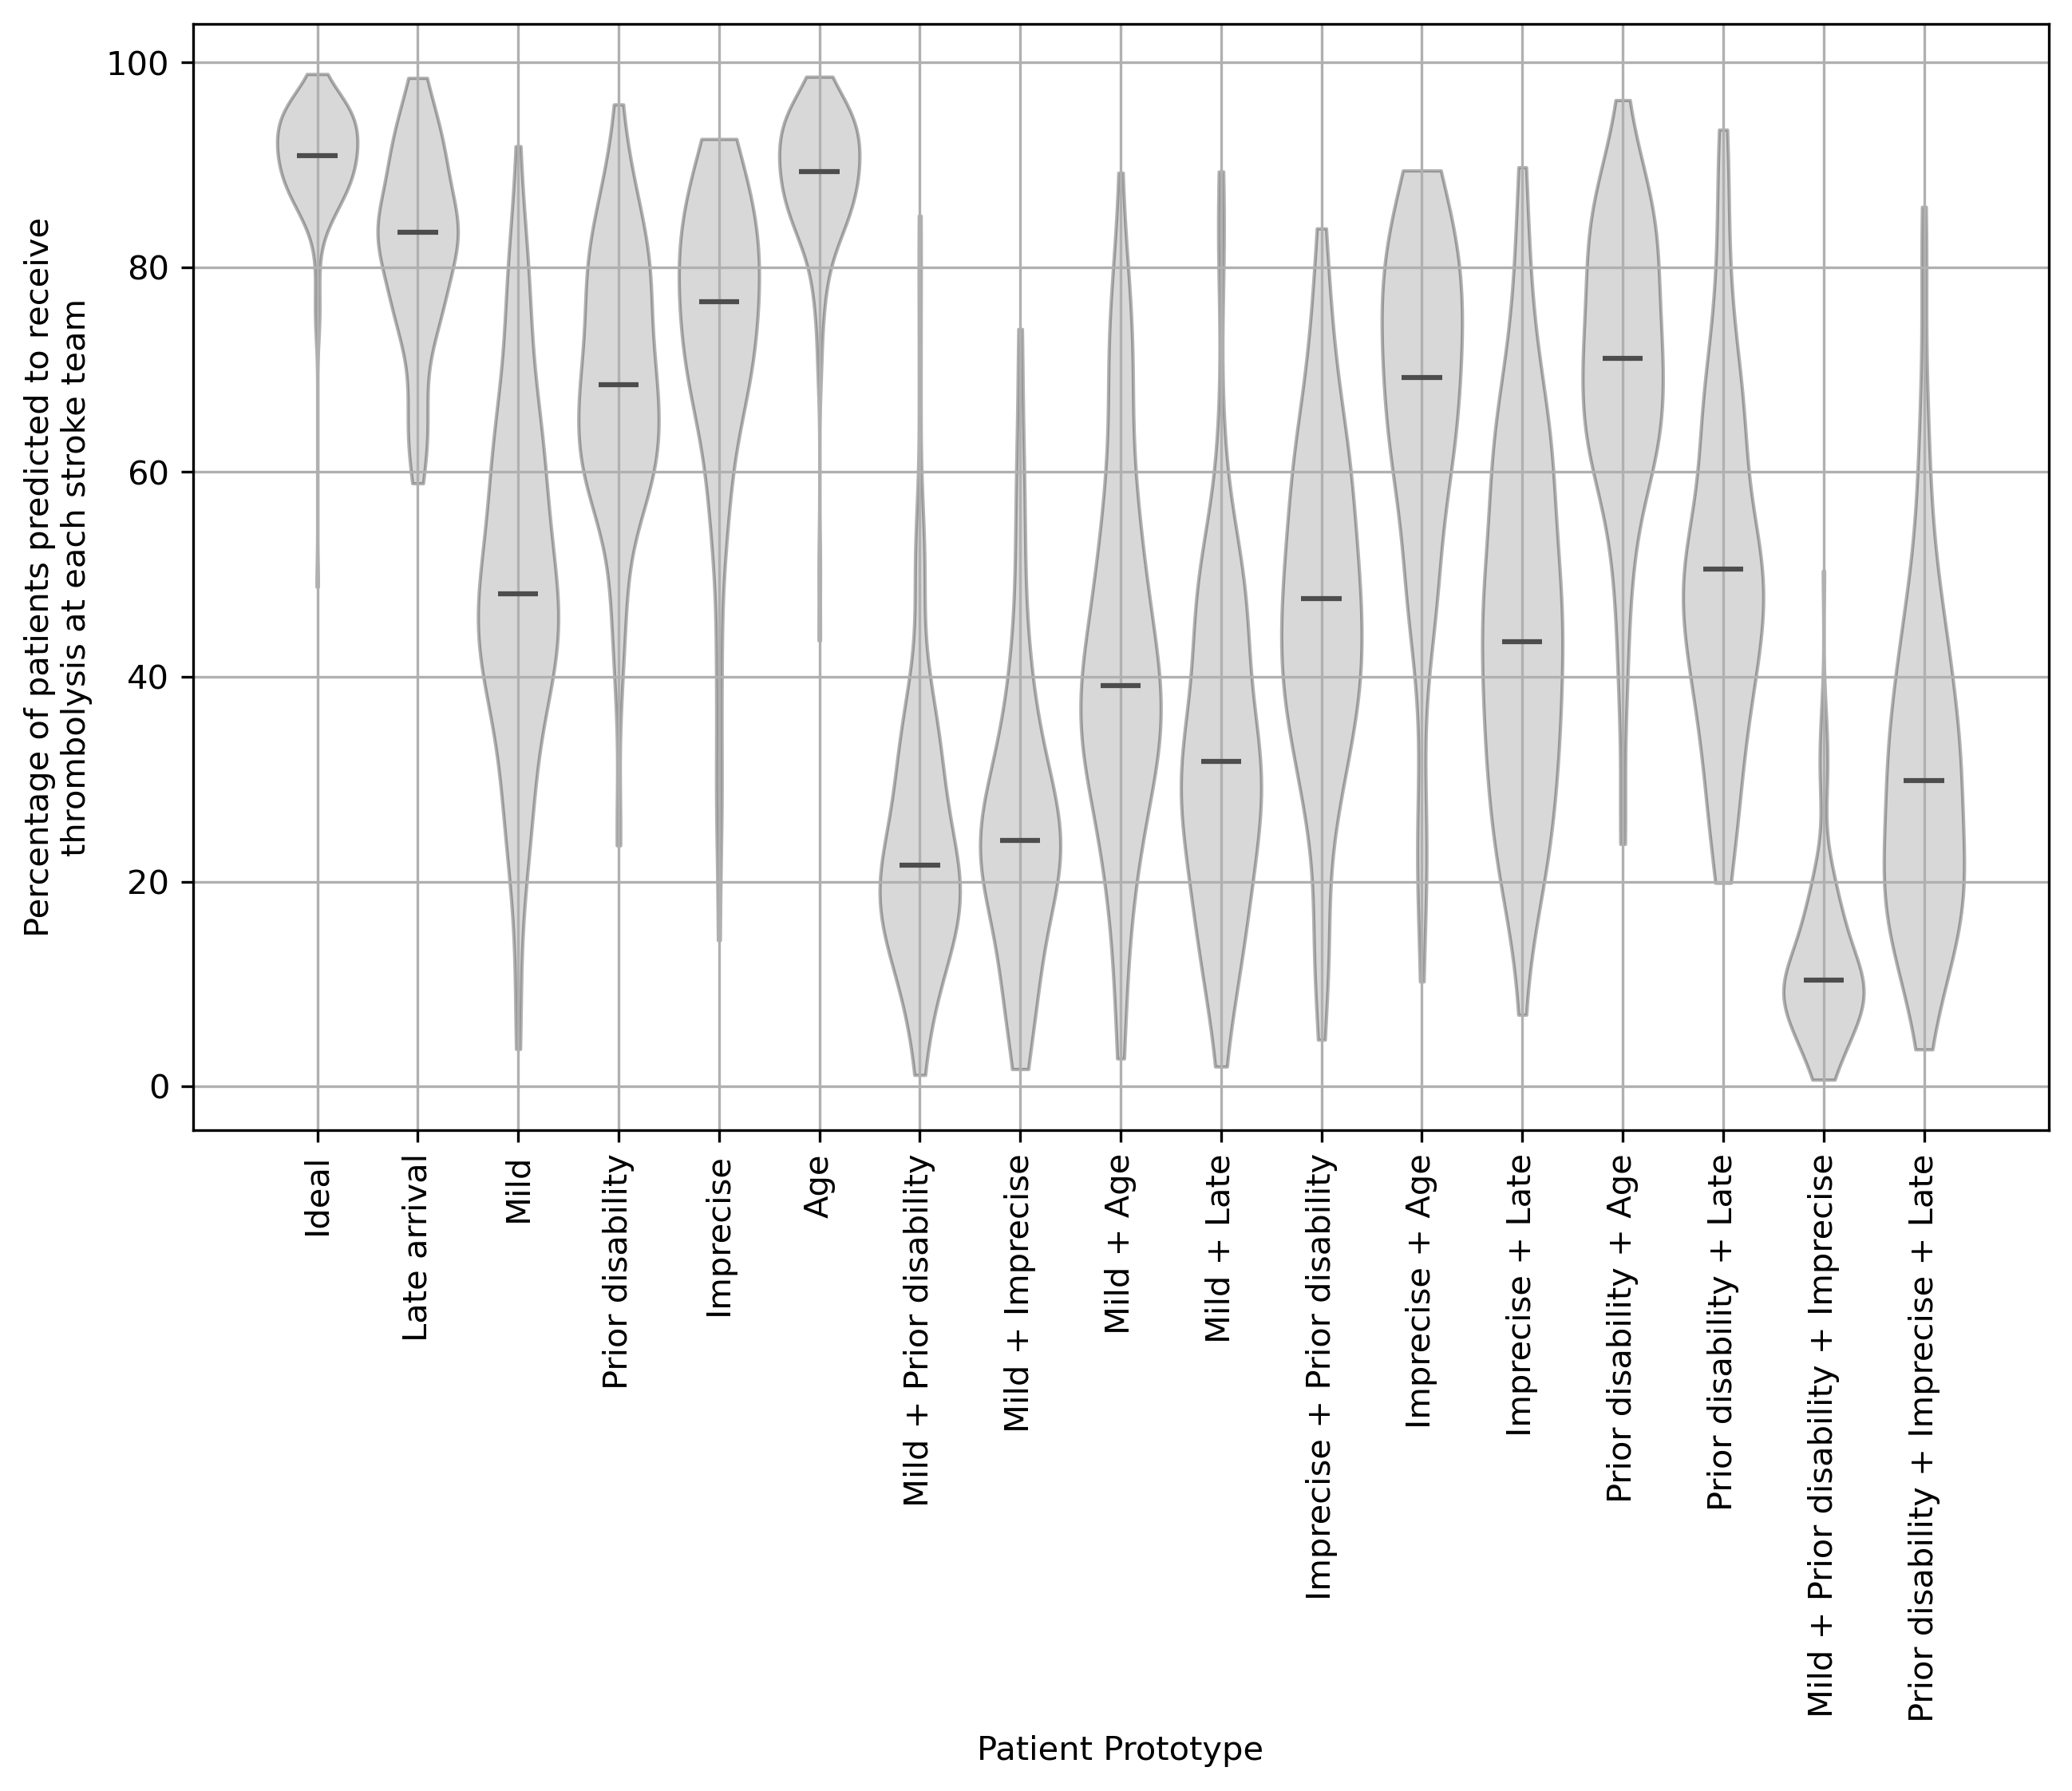
\includegraphics[width=0.75\linewidth]{images/prototype_patients_all_teams}
    \caption{Violin plots showing the variation in predicted thrombolysis rates for 17 patient prototypes across stroke teams. \textit{Ideal}: Onset-to-arrival = 90 minutes; arrival-to-scan = 15 minutes; onset-to-thrombolysis = 120 minutes; stroke severity (NIHSS) = 15; pre-stroke disability (mRS) = 0; age = 72.5; Precisely known onset; onset not during sleep; stroke type = Infarction; patient has no atrial fibrillation and is not receiving anticoagulants for atrial fibrillation; \textit{Late arrival}: as \textit{ideal} but onset-to-arrival = 225 minutes and onset-to-thrombolysis = 255 minutes \textit{Mild}: As \textit{ideal} but stroke severity = 3; \textit{Prior disability}: as \textit{ideal} but pre-stroke disability = 3; \textit{Imprecise}: as \textit{ideal} but stroke onset time estimated; \textit{Age}: as \textit{ideal} but age = 87.5.}
    \label{fig:thrombolysis_rates_prototype_patients}
\end{figure}

Figure \ref{fig:thrombolysis_rates_prototype_patients_team_x} shows an example of thrombolysis decisions for prototype patients in one stroke team, which is especially unlikely to give thrombolysis to patients with mild stroke, comparing likely use of thrombolysis to \textit{benchmark} hospitals.

\begin{figure}
    \centering
    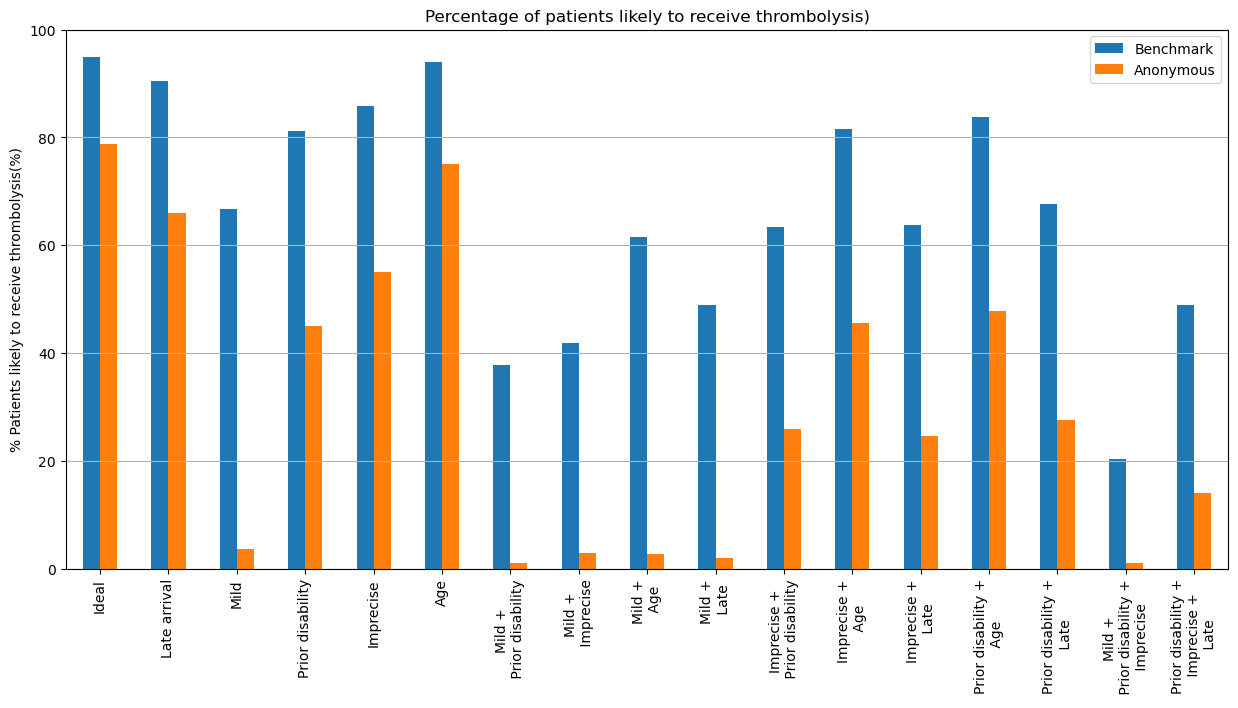
\includegraphics[width=1\linewidth]{images/prototype_patients_team_x.png}
    \caption{Predicted use of thrombolysis in 17 patient prototypes at a single hospital. Results show the the percentage of patients likely to receive thrombolysis, comparing \textit{benchmark decisions} (blue) and decisions likely at the example hospital (orange). Patient prototypes were: \textit{Ideal} candidate characteristics: Onset-to-arrival = 90 minutes; arrival-to-scan = 15 minutes; onset-to-thrombolysis = 120 minutes; stroke severity (NIHSS) = 15; pre-stroke disability (mRS) = 0; age = 72.5; precisely known onset; onset not during sleep; stroke type = infarction; patient has no atrial fibrillation and is not receiving anticoagulants for atrial fibrillation. Patient with mild stroke is as \textit{ideal} candidate, but with NIHSS = 3.}
    \label{fig:thrombolysis_rates_prototype_patients_team_x}
\end{figure}


\subsubsection{Expected outcomes in prototype patients}

Figure \ref{fig:example_patient_outcomes} shows examples of outcome prediction for an \textit{ideal} candidate for thrombolysis, and a patient who is otherwise the same but has mild stroke. Expected benefit from thrombolysis may be calculated as the change in the proportion of \textit{good outcomes} (e.g. mRS 0-2), the proportion of \textit{bad outcomes} (e.g. mRS 5-6), or the shift in the central point of the outcome distribution (by weighting each mRS level by the probability of being discharged with that level of disability). 


\begin{figure}[h]
    \centering
    \begin{subfigure}[b]{1.0\textwidth}
        \centering
    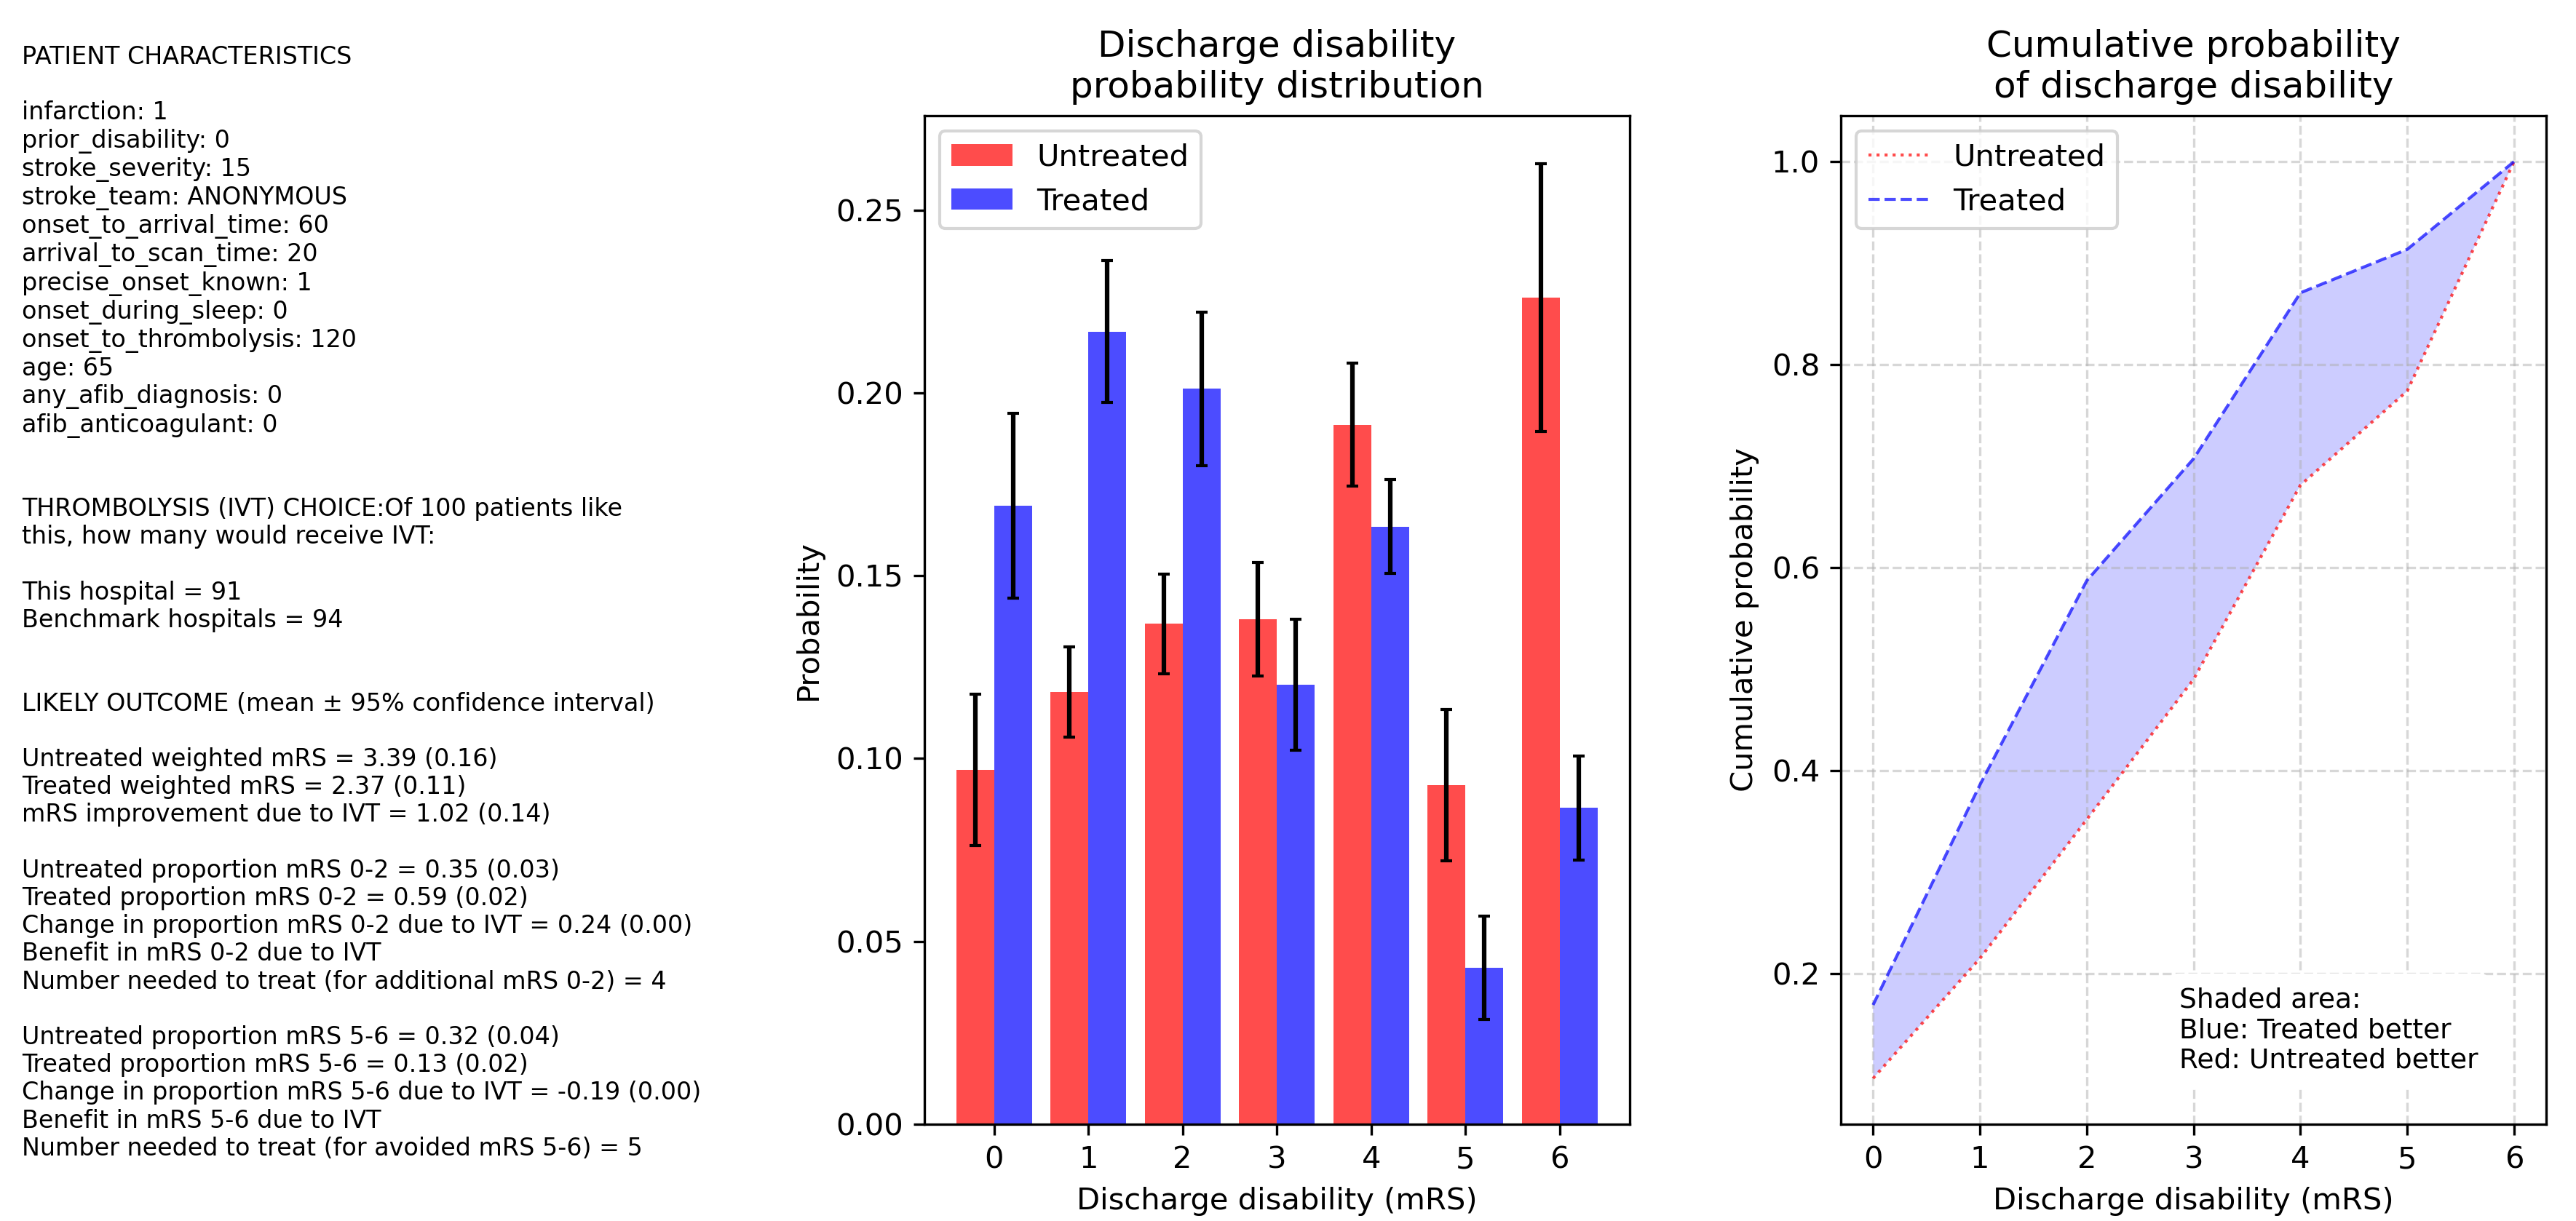
\includegraphics[width=1.0\linewidth]{images/prototype_patient_ideal}
        \caption{\textit{Ideal} candidate for thrombolysis}
        \label{fig:patient_outcome_subfig1}
    \end{subfigure}
    \\
    \vspace{8mm}
    \begin{subfigure}[b]{1.0\textwidth}
        \centering
        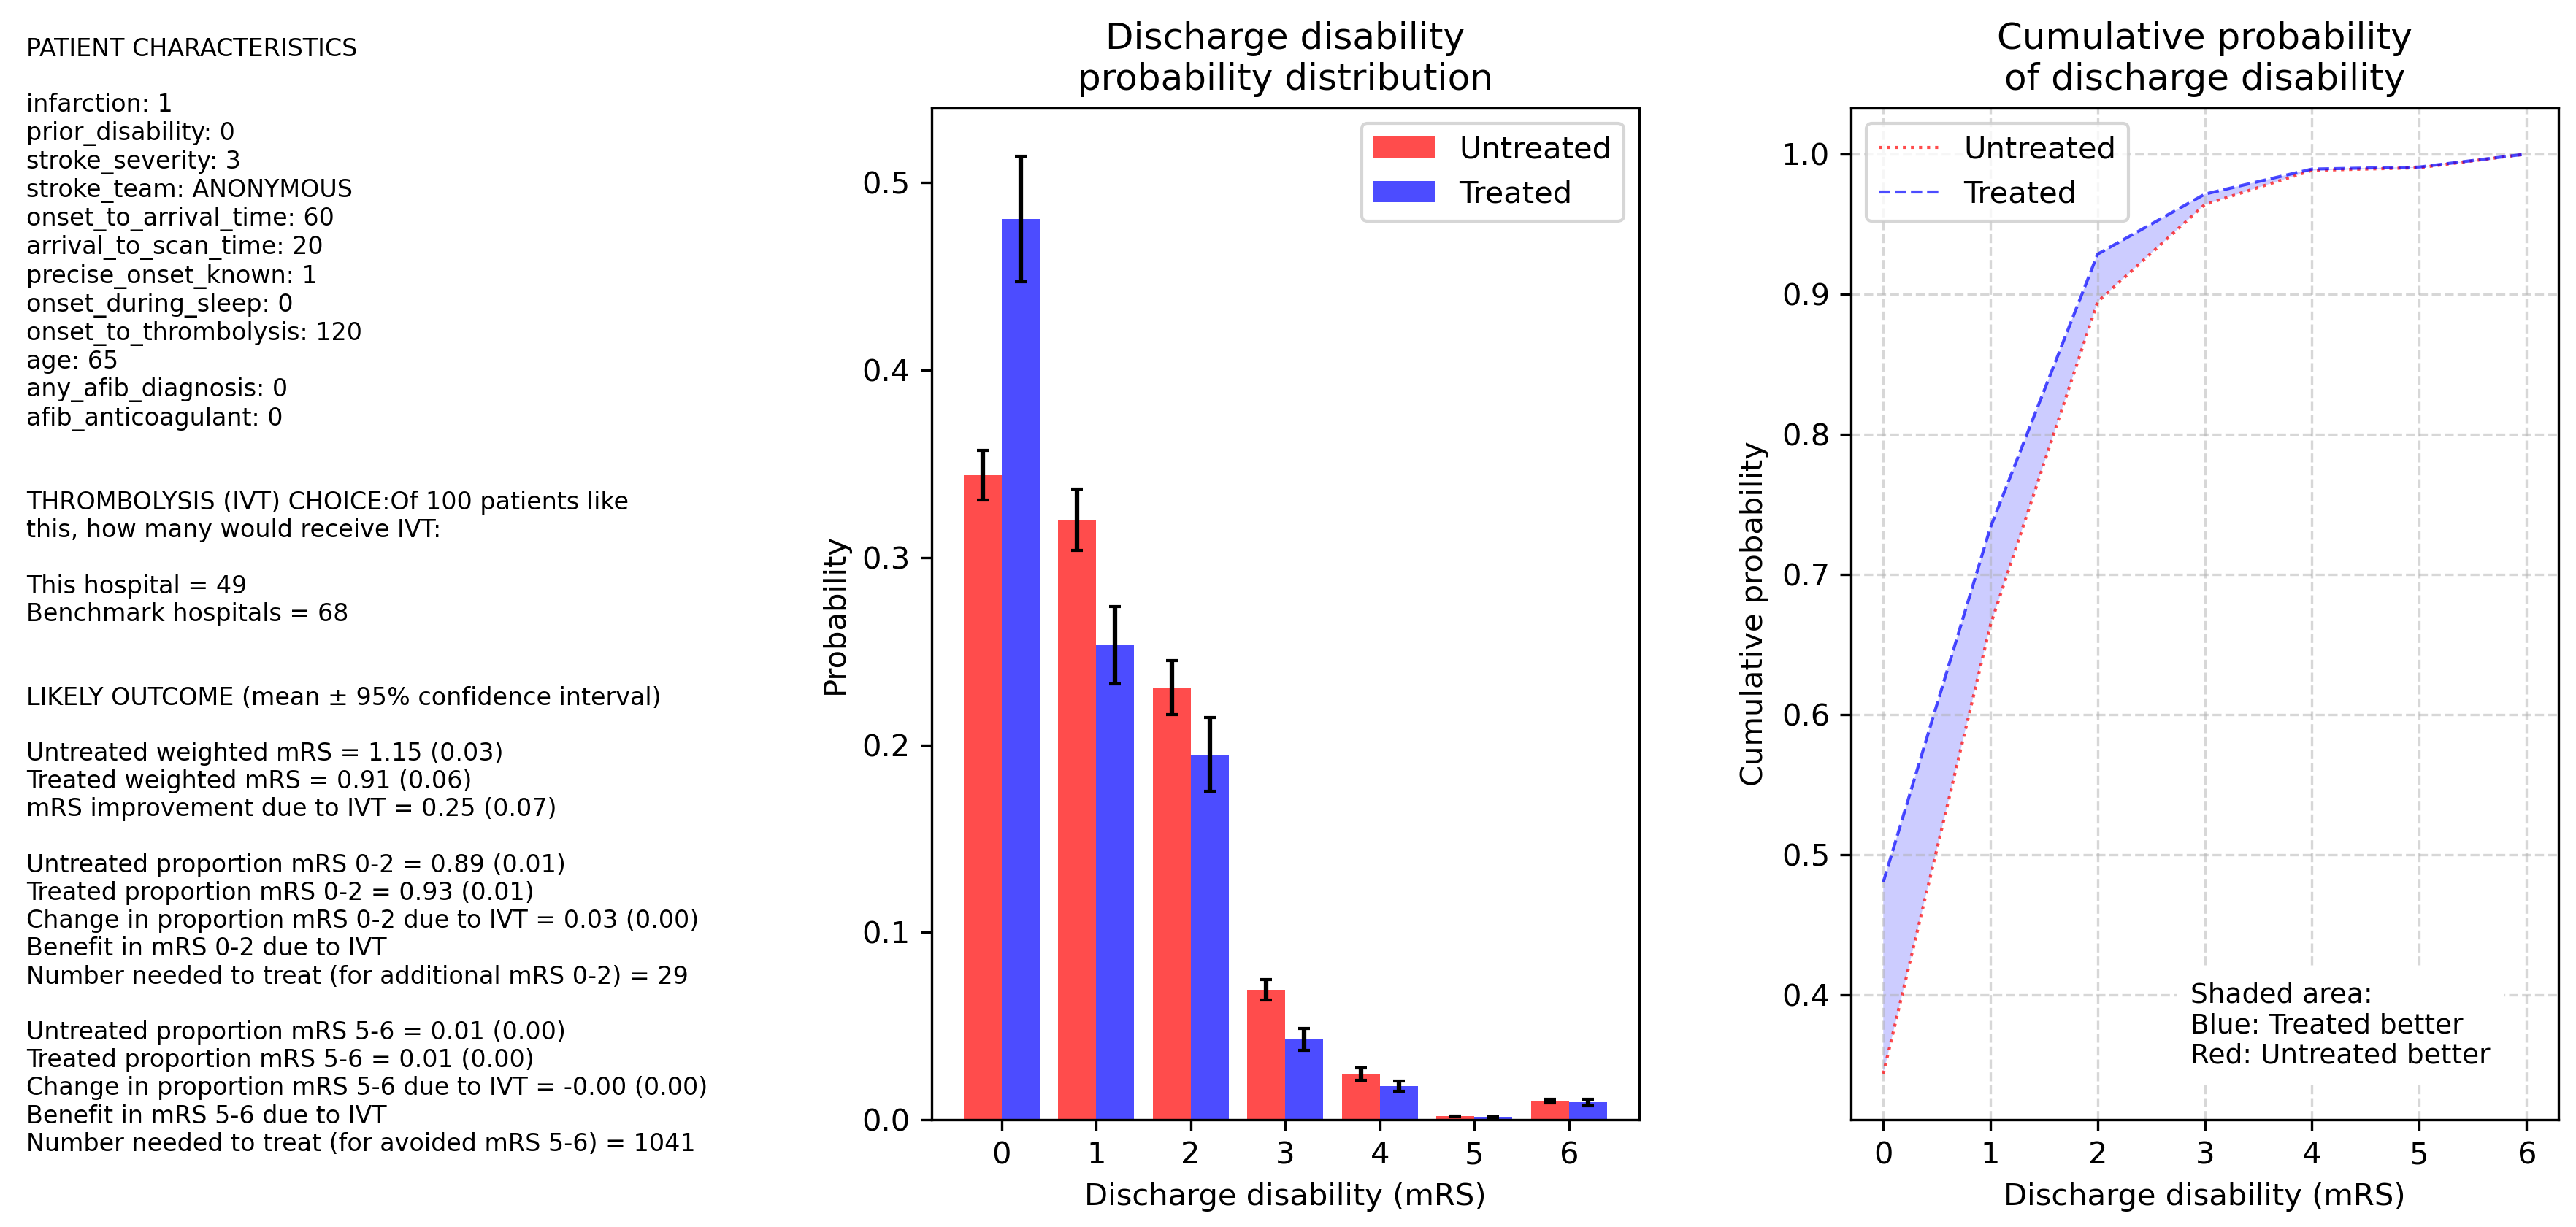
\includegraphics[width=1.0\linewidth]{images/prototype_patient_mild}
        \caption{Patient as \textit{Ideal} candidate for thrombolysis, but with mild stroke (NIHSS 3)}
        \label{fig:patient_outcome_subfig2}
    \end{subfigure}
    \caption{Predicted outcome probabilities, with and without thrombolysis, for an \textit{ideal} candidate for thrombolysis (top) and for a patient with mild stroke (bottom). \textit{Ideal} candidate characteristics: Onset-to-arrival = 90 minutes; arrival-to-scan = 15 minutes; onset-to-thrombolysis = 120 minutes; stroke severity (NIHSS) = 15; pre-stroke disability (mRS) = 0; age = 72.5; Precisely known onset; onset not during sleep; stroke type = Infarction; patient has no atrial fibrillation and is not receiving anticoagulants for atrial fibrillation. Patient with mild stroke is as \textit{ideal} candidate, but with NIHSS = 3. Errors shown are 95\% confidence limits derived from 30 bootstrapped models.}
    \label{fig:example_patient_outcomes}
\end{figure}



Table \ref{tab:prototype_outcomes} shows predicted outcomes across all prototype patients. All these patients would likely benefit from thrombolysis, but the benefit in mild stroke was smaller.

\begin{minipage}{1\textwidth}
\small
\begin{longtable}{p{5.2cm} | p{1.6cm} p{1.6cm} p{1.5cm} | p{1.6cm} p{1.6cm} p{1.5cm}}
\caption{Predicted outcomes for patient prototypes. \textit{Ideal}: Onset-to-arrival = 90 minutes; arrival-to-scan = 15 minutes; onset-to-thrombolysis = 120 minutes; stroke severity (NIHSS) = 15; pre-stroke disability (mRS) = 0; age = 72.5; precisely known onset; onset not during sleep; stroke type = infarction; patient has no atrial fibrillation and is not receiving anticoagulants for atrial fibrillation. \textit{Late arrival}: as \textit{ideal} but onset-to-arrival = 225 minutes and onset-to-thrombolysis = 255 minutes. \textit{Mild}; As \textit{ideal} but stroke severity = 3; \textit{Prior disability}: as \textit{ideal} but pre-stroke disability = 3; \textit{Imprecise}: as \textit{ideal} but stroke onset time estimated. \textit{Age}: as \textit{ideal} but age = 87.5. Results show probability-weighted disability at discharge, and the proportion of patients predicted to have a very poor outcome (mRS 5-6).}\\
\label{tab:prototype_outcomes}
Patient prototype & Untreated probability-weighted mRS & Treated probability-weighted mRS & Improve-ment & Untreated proportion mRS 5-6 & Treated proportion mRS 5-6 & Improve-ment\\
\endhead
\midrule
Ideal & 3.39 & 2.37 & 1.02 & 0.32 & 0.13 & 0.19\\
Late & 3.39 & 2.73 & 0.66 & 0.32 & 0.18 & 0.14\\
Mild & 1.15 & 0.91 & 0.23 & 0.01 & 0.01 & 0.00\\
Prior disability & 4.22 & 3.61 & 0.61 & 0.41 & 0.23 & 0.19\\
Imprecise & 3.49 & 2.39 & 1.10 & 0.33 & 0.13 & 0.20\\
Age & 4.22 & 3.51 & 0.71 & 0.50 & 0.35 & 0.16\\
Mild + Prior disability & 2.92 & 2.60 & 0.32 & 0.04 & 0.04 & 0.00\\
Mild + Imprecise & 1.28 & 1.01 & 0.26 & 0.02 & 0.01 & 0.00\\
Mild + Age & 1.84 & 1.63 & 0.22 & 0.04 & 0.03 & 0.01\\
Mild + Late & 1.15 & 0.77 & 0.39 & 0.01 & 0.00 & 0.00\\
Imprecise + Prior disability & 4.33 & 3.67 & 0.66 & 0.44 & 0.24 & 0.20\\
Imprecise + Age & 4.31 & 3.57 & 0.74 & 0.53 & 0.36 & 0.17\\
Imprecise + Late & 3.49 & 2.75 & 0.74 & 0.33 & 0.17 & 0.17\\
Prior disability + Age & 4.62 & 4.35 & 0.27 & 0.53 & 0.44 & 0.08\\
Prior disability + Late & 4.22 & 3.70 & 0.52 & 0.41 & 0.27 & 0.14\\
Mild + Prior disability + Imprecise & 3.01 & 2.65 & 0.36 & 0.06 & 0.06 & 0.00\\


\end{longtable}
\normalsize
\end{minipage}

\subsection{Mild stroke}

Table \ref{tab:mild_stroke} shows the predicted benefit of thrombolysis in mild ischaemic stroke (NIHSS 0-4) and non-mild stroke (NIHSS 5+). If thrombolysis were given to all mild stroke patients, the outcome model predicted that the proportion of patients with good outcomes (mRS 0-1 or -2) would reduce, the proportion with bad outcome (mRS 5-6) would increase and there would be a worsening in average mRS. In those mild stroke patients who actually received thrombolysis, either at a benchmark hospital or a non-benchmark hospital, it was predicted that there would be an increased proportion of good outcomes, and a beneficial shift in average mRS. The model predicted that in these groups there would still be a small increase in bad outcomes, but this was reduced to use in all mild stroke admissions. In non-mild stroke, thrombolysis had a net benefit by all measures in all groups.


\begin{minipage}{1\textwidth}
\small
\renewcommand{\arraystretch}{1.2}
\begin{longtable}{p{7.2cm} | p{1.6cm} p{1.6cm} | p{1.6cm} p{1.6cm}}
\caption{Patient characteristics and predicted outcomes for mild stroke (NIHSS 0-4) and non-mild stroke (NIHSS 5+). Results shown are the mean for all patients who actually received treatment at either a non-benchmark hospital or a benchmark hospital.}\\
\label{tab:mild_stroke}

Metric & Non-benchmark NIHSS 0-4 & Non-benchmark NIHSS 5+ & Benchmark NIHSS 0-4 & Benchmark NIHSS 5+\\
\endhead
\midrule
Stroke severity & 3.1 & 12.8 & 2.9 & 12.5\\
Onset to thrombolysis (minutes) & 147 & 138 & 140 & 130\\
Proportion onset known precisely & 86\% & 84\% & 77\% & 71\%\\
Proportion untreated mRS 0-1 & 0.556 & 0.240 & 0.564 & 0.234\\
Proportion untreated mRS 0-2 & 0.797 & 0.401 & 0.795 & 0.399\\
Proportion untreated mRS 5-6 & 0.026 & 0.281 & 0.024 & 0.284\\
Untreated weighted mRS & 1.535 & 3.188 & 1.537 & 3.205\\
Change in proportion mRS 0-1 (+ve is better) & 0.019 & 0.063 & 0.027 & 0.072\\
Change in proportion mRS 0-2 (+ve is better) & 0.012 & 0.079 & 0.009 & 0.078\\
Change in proportion mRS 5-6 (-ve is better) & 0.010 & -0.056 & 0.009 & -0.057\\
Change in weighted mRS ( -ve is better) & -0.036 & -0.341 & -0.053 & -0.354\\

\end{longtable}
\normalsize
\end{minipage}


\subsection{Lifetime economic model}

Table \ref{tab:health_econ} shows the modelled health economics of thrombolysis use, comparing actual use of thrombolysis with \textit{benchmark} thrombolysis use. Benchmark decisions maintain the benefit of using thrombolysis, but extend that benefit to more patients. This extended benefit was not at the cost of any predicted increase in the worst outcomes (mRS 5-6). The extended benefit led to more QALYs added across the population by treatment, and more predicted savings to NHS healthcare costs.

\begin{table}[!h]
\small
\caption{Health economic analysis: Analysis for  populations based on predicted benefit (or dis-benefit) of thrombolysis. The analysis compares the populations currently treated, or the population that would be treated using \textit{benchmark} decisions (the majority vote of the predicted choice of the the 25 stroke teams most likely to use thrombolysis). Results are shown for (a) the treated populations, and (b) adjusted for 1,000 emergency stroke admissions }
\label{tab:main}

\begin{subtable}{1\textwidth}
\centering
\caption{Counterfactual analysis of the effect of thrombolysis in either those patients who actually received thrombolysis, or those patients where the \textit{benchmark decision} would be to use thrombolysis.}
\begin{tabular}{p{2.0cm} p{1.4cm} p{1.3cm} p{1.3cm} p{1.5cm} p{1.3cm} p{1.4cm} p{1.3cm} p{1.3cm}}
\toprule
Population & \raggedright Treated or not treated & Death & Survival (median years) & Care years (median) & QALYs & \raggedright Discounted cost per patient & Proportion mRS 0-2 & Proportion mRS 5-6\tabularnewline
\midrule
Actual & Untreated & 17.1\% & 7.60 & 0.28 & 5.020 & £20,370 & 47.1\% & 23.9\%\tabularnewline
& Treated & 14.2\% & 7.91 & 0.25 & 5.258 & £19,806 & 53.9\% & 19.3\%\tabularnewline
& Difference & -2.9\% & 0.31 & -0.03 & 0.238 & -£565 & 6.8\% & -4.7\%\tabularnewline
\midrule
Benchmark & Untreated & 17.4\% & 7.63 & 0.28 & 5.036 & £20,388 & 46.5\% & 24.1\%\tabularnewline
& Treated & 14.4\% & 7.93 & 0.25 & 5.269 & £19,784 & 53.4\% & 19.4\%\tabularnewline
& Difference & -3.0\% & 0.30 & -0.03 & 0.234 & -£603 & 6.9\% & -4.8\%\tabularnewline

\end{tabular}
\end{subtable}

\vspace{3mm}

\begin{subtable}{1\textwidth}
\centering
\caption{Analysis for 1,000 emergency stroke admissions (all stroke types)}
\begin{tabular}{p{1.9cm} p{1.9cm} p{1.9cm} p{1.9cm} p{1.9cm} p{1.9cm} p{2.2cm}}
\toprule
Population & Proportion treated & QALYs added & Healthcare costs saved & \raggedright Thrombolysis cost (£450 per patient) & \raggedright Cost per QALY added & \raggedright Net cost of thrombolysis\tabularnewline
\midrule
Actual & 11.0\% & 26.3 & £62,294 & £49,658 & £1,890 & -£12,637\tabularnewline
Benchmark & 13.6\% & 31.7 & £81,914 & £61,117 & £1,927 & -£20,797\tabularnewline
\bottomrule
\end{tabular}
\end{subtable}
\label{tab:health_econ}
\end{table}

\normalsize

\subsection{Pathway model}

Figure \ref{fig:thrombolysis_rates_teams} compares observed and predicted thrombolysis use (based on historic performance, and applying \textit{benchmark decisions}). Predicted and observed thrombolysis use correlate very closely (r-squared 0.94). Predicted rates were, on average, slightly higher (1.7\%) than observed rates.

\begin{figure}[!h]
    \centering
    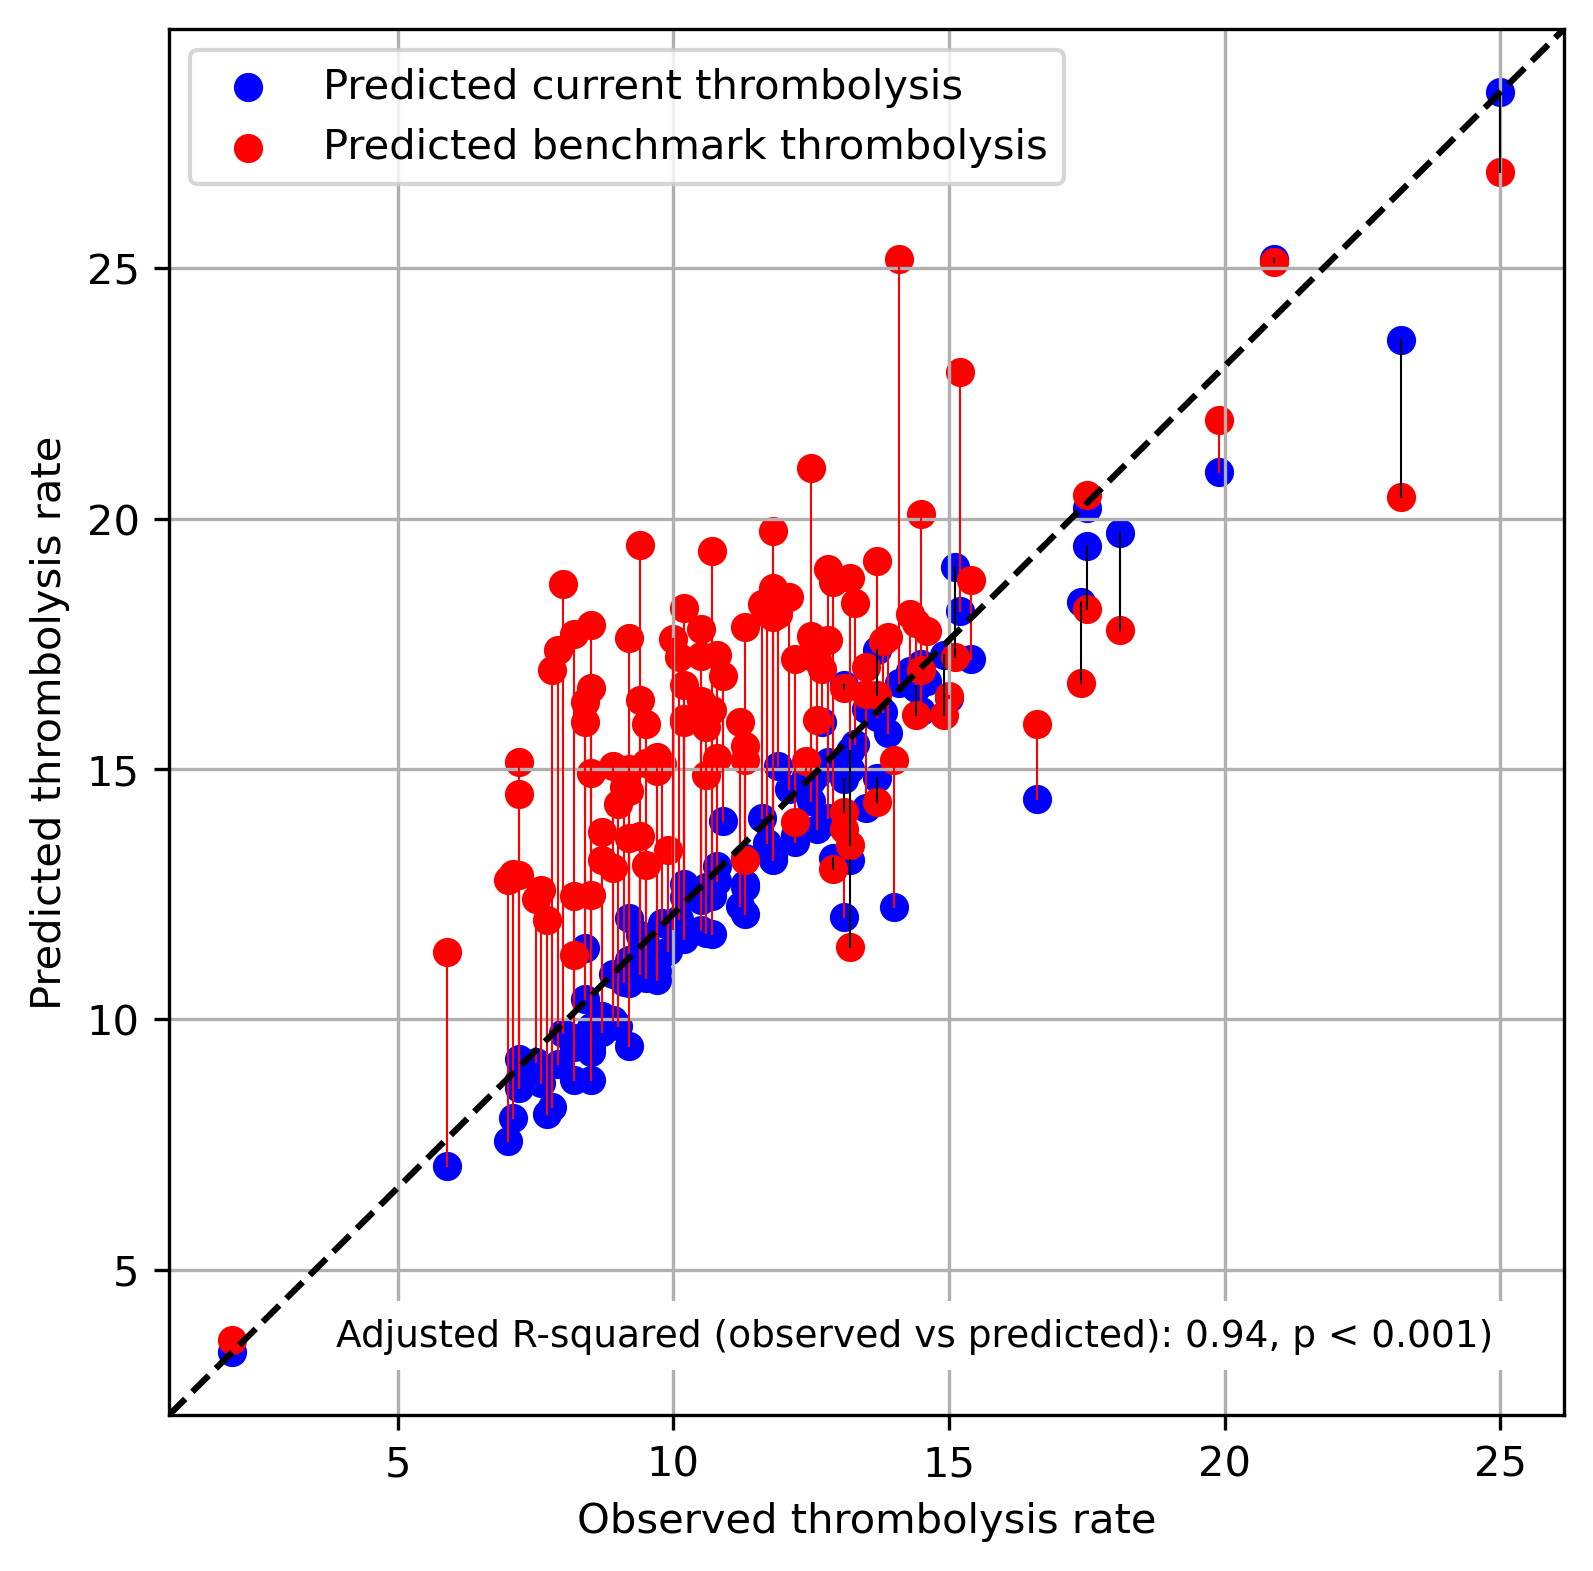
\includegraphics[width=0.5\linewidth]{images/thrombolysis_rates_model}
    \caption{Comparison of observed and predicted thrombolysis use across stroke teams. Blue circles show predictions based on historic hospital performance. Red circles show the expected thrombolysis use if \textit{benchmark decisions} were made. The black dotted line shows least-squares regression analysis between observed and predicted (using historic performance) thrombolysis use.}
    \label{fig:thrombolysis_rates_teams}
\end{figure}


Across the study population, by combining pathway improvements, thrombolysis use in all those emergency stroke admissions arriving by ambulance shows the potential to be increased from 13\% to 20\% (figure \ref{fig:scenarios_population}). Using a model based on clinical trial data, benefit, as measured by number of number of people discharged with no, or minimal, disability (mRS 0 or 1)  could be doubled from 10 to 20 additional excellent outcomes per 1,000 admissions. The single most influential change was applying \textit{benchmark} decisions. Improving speed would not significantly increase the number of people given thrombolysis, but would lead to more benefit from thrombolysis (as all treated patients will have improved benefit). Figure \ref{fig:scenarios_team} shows this analysis applied to a single stroke team.


\begin{figure}[!h]
    \centering
    \begin{subfigure}[b]{1\textwidth}
        \centering
        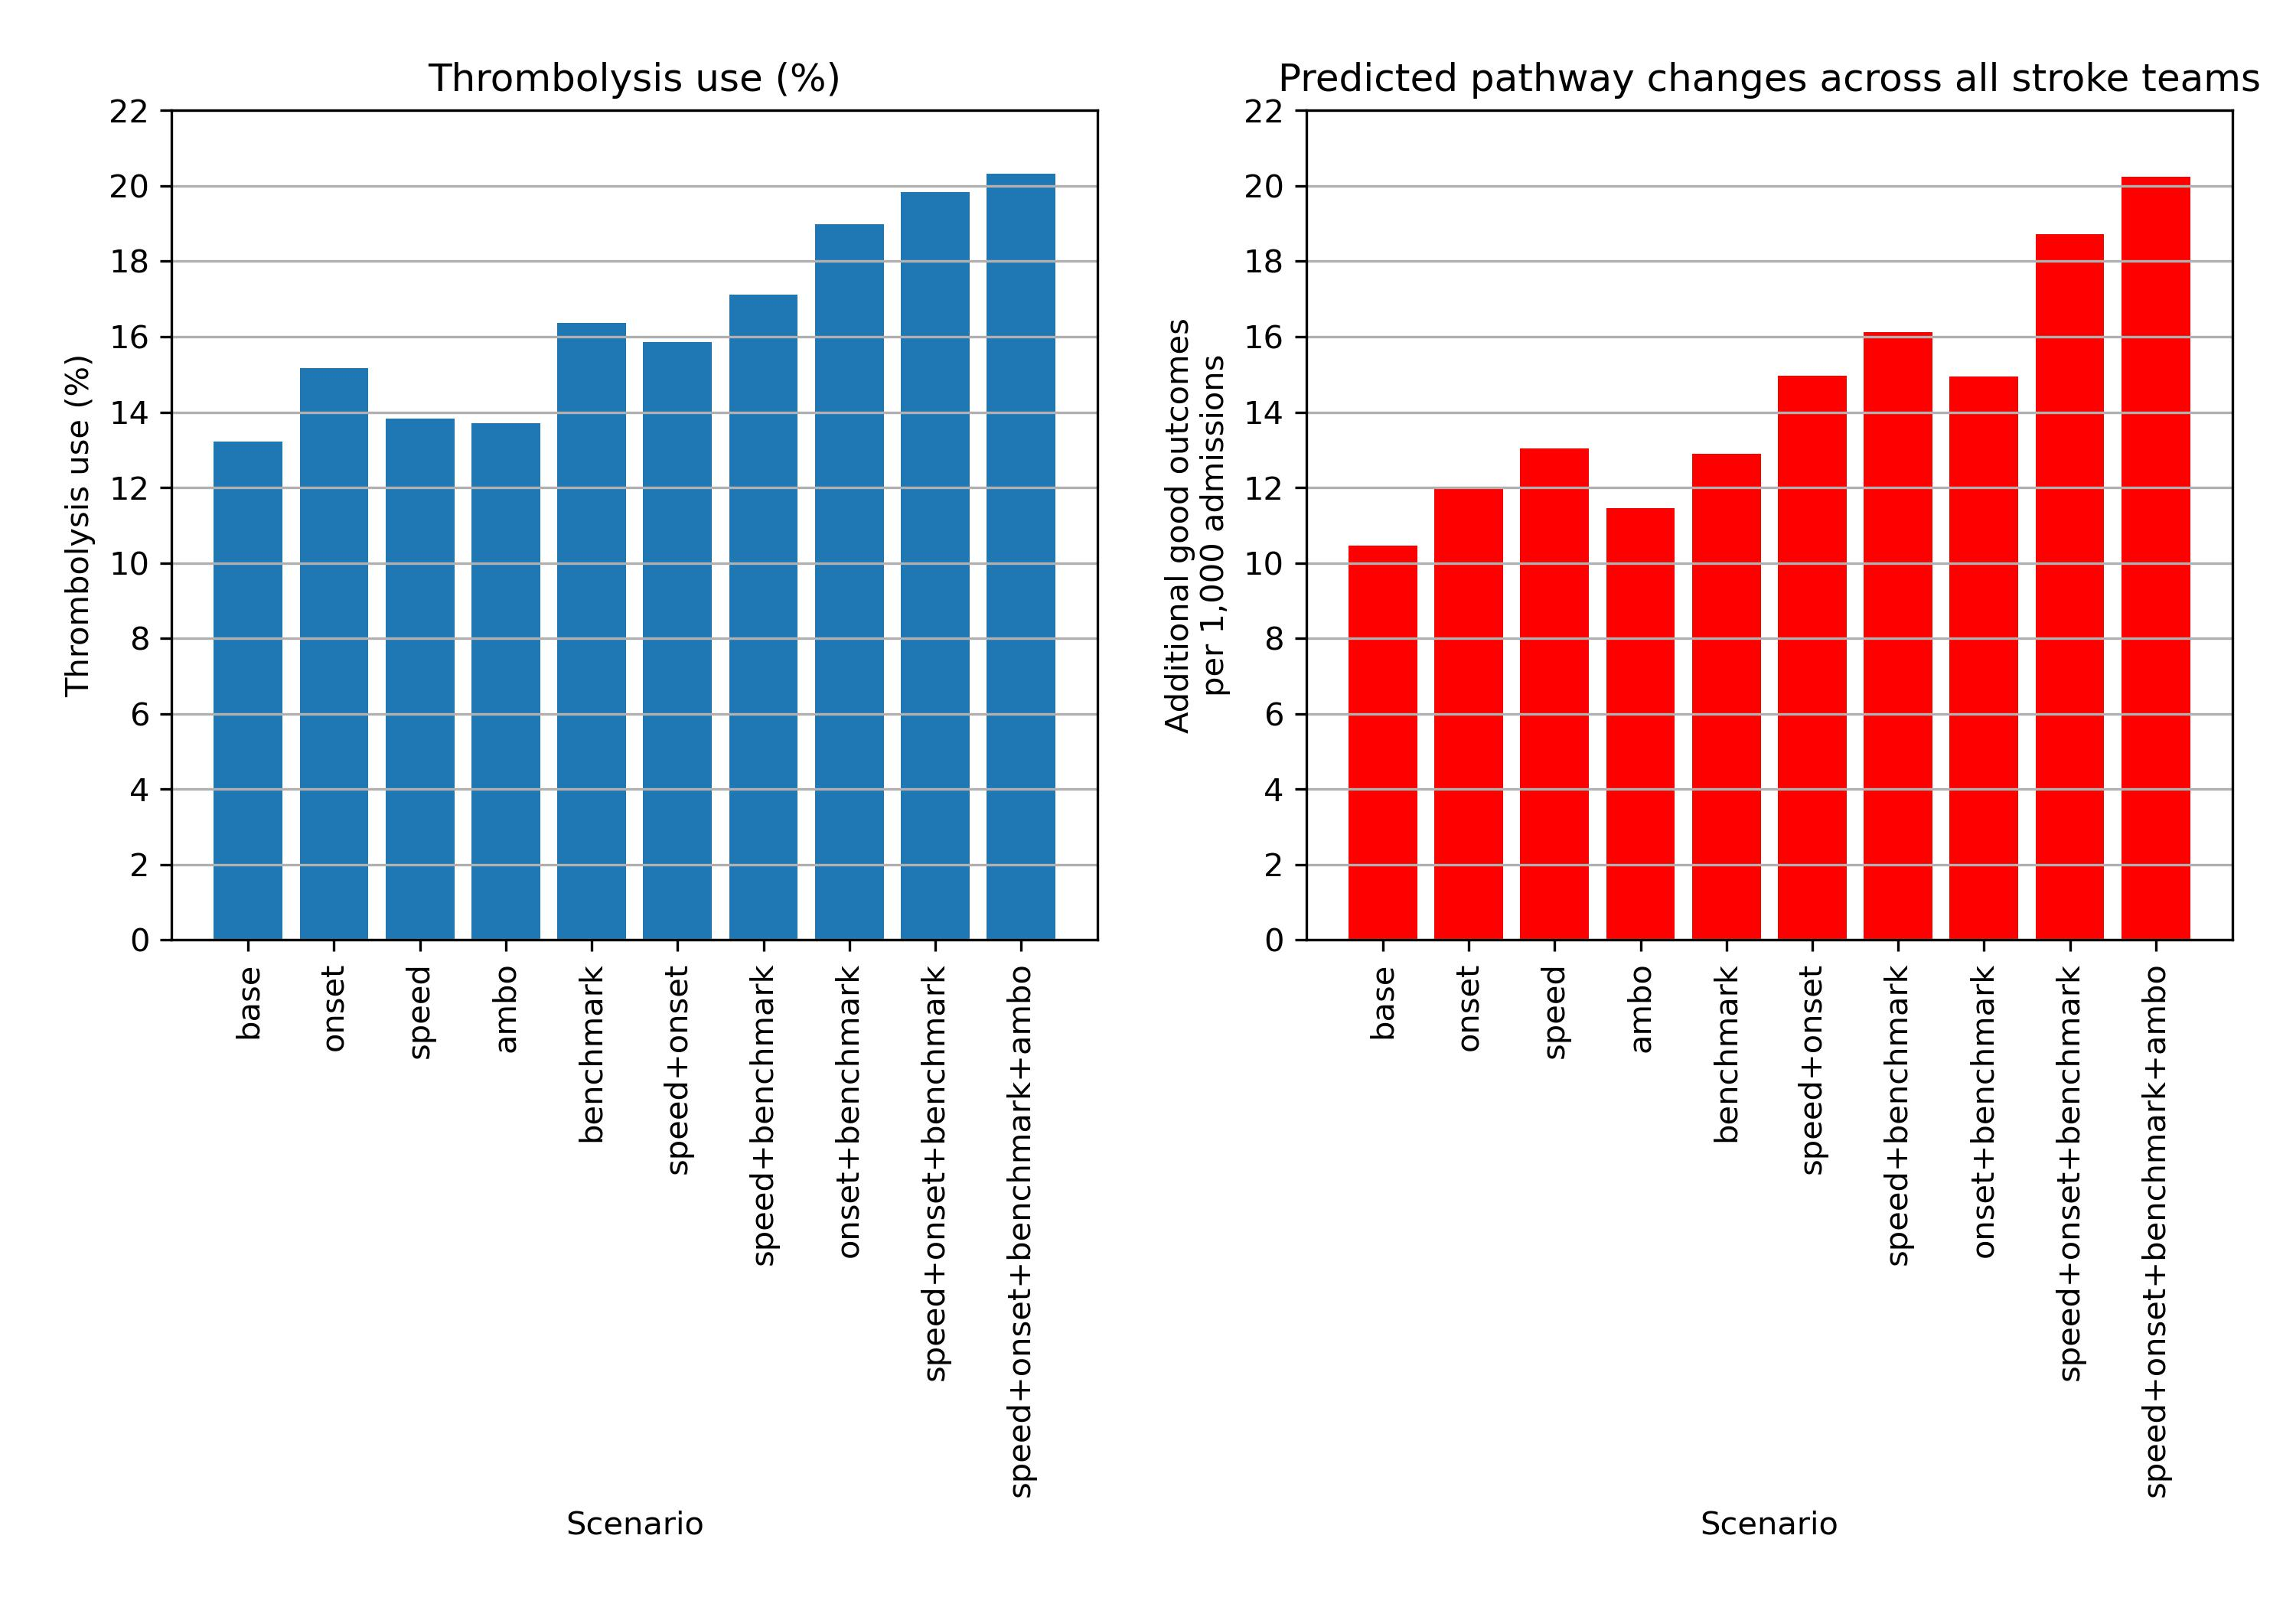
\includegraphics[width=0.8\linewidth]{images/sim_results_summary}
        \caption{Changes across the study population}
        \label{fig:scenarios_population}
    \end{subfigure}
    \\
    \vspace{8mm}
    \begin{subfigure}[b]{1\textwidth}
        \centering
    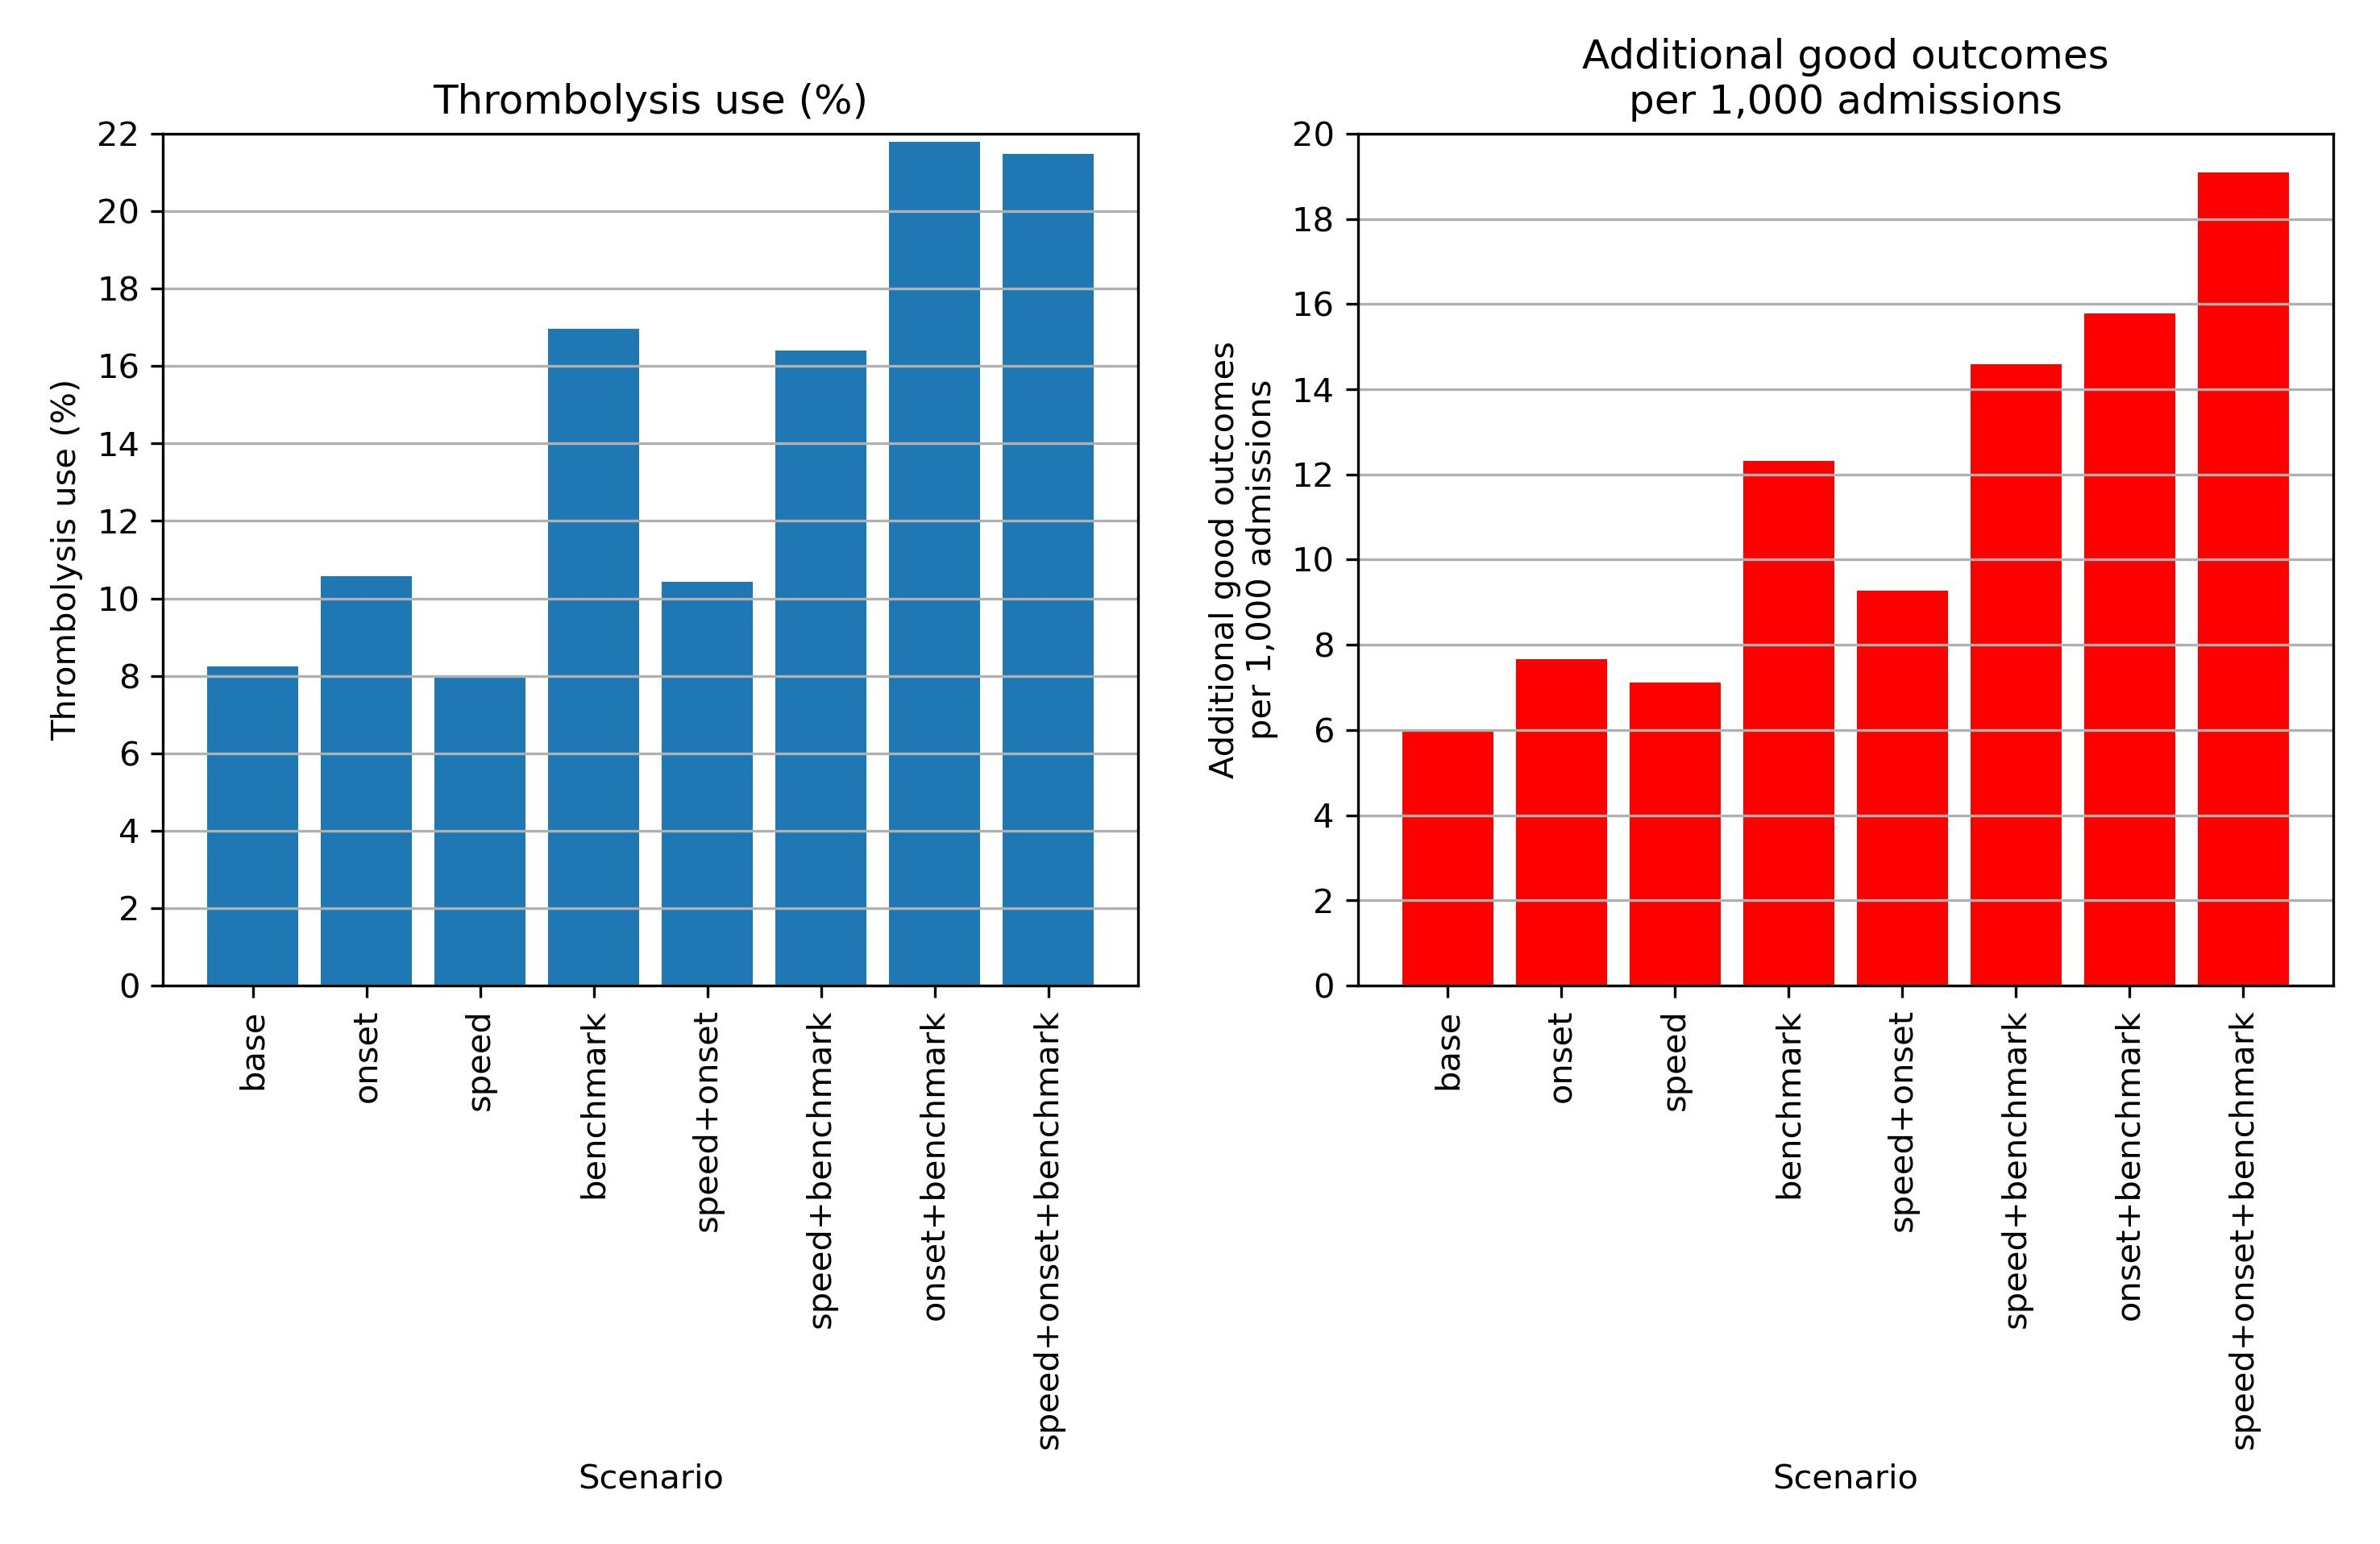
\includegraphics[width=0.8\linewidth]{images/sim_results_team_x}
        \caption{Changes in one stroke team}
        \label{fig:scenarios_team}
    \end{subfigure}
    \caption{Expected effect of alternative process improvement initiatives across the study population (top) or one specific stroke team (bottom). Each chart shows the effect on thrombolysis use (left) and on number of additional good outcomes (mRS 0-1) per 1,000 admissions due to use of thrombolysis (right). \textit{Base}: Uses the hospitals’ recorded pathway statistics. \textit{Speed}: Sets 95\% of patients having a scan within 4 hours of arrival, and all patients have 15 minutes arrival-to-scan time and 15 minutes scan-to-needle time.\textit{Ambo}: Subtracts 15 minutes from the current ambulance call to arrival-at-hospital times. \textit{Onset-known}: Sets the proportion of patients with a known stroke onset time to the national upper quartile if currently less than the national upper quartile. \textit{Benchmark}: The benchmark thrombolysis rate takes the likelihood to give thrombolysis for patients scanned within 4 hours of onset from the majority vote of the 25 benchmark hospitals.}
    \label{fig:sim_results_summary}
\end{figure}


